\documentclass[letterpaper,12pt,fleqn]{article}
\usepackage{matharticle}
\usepackage{enumitem}
\pagestyle{plain}
\newcommand{\cycle}[1]{\left<#1\right>}
\newcommand{\n}{\mathrel{\triangleleft}}
\renewcommand{\o}{\sigma}
\renewcommand{\t}{\tau}
\newcommand{\p}{\phi}
\begin{document}
Cavallaro, Jeffery \\
Math 221a \\
Homework \#4

\bigskip

\subsection*{1.4.2}
\begin{enumerate}[label={\alph*)}]
\item Let $H$ be the cyclic subgroup (of order 2) of $S_3$ generated by
  $(12)$. \\
  Prove: No left coset of $H$ (except $H$ itself) is also a right coset.

  $S_3=\{(),(12),(13),(23),(123),(132)\}$ \\
  $H=\{(),(12)\}$

  \begin{minipage}[t]{2.5in}
    $()H=\{(),(12)\}=H$ \\
    $(13)H=\{(13),(123)\}$ \\
    $(23)H=\{(23),(132)\}$
  \end{minipage}
  \begin{minipage}[t]{2.5in}
    $H()=\{(),(12)\}=H$ \\
    $H(13)=\{(13),(132)\}$ \\
    $H(23)=\{(23),(123)\}$
  \end{minipage}

  Thus, no left coset matches a right coset (other than $H$).

  Prove: $\exists\,a\in S_3,aH\cap Ha=\{a\}$

  Let $a=(13)$ \\
  $(13)H\cap H(13)=(13)$

\item Prove: If $K$ is the cyclic group (of order 3) generated by $(123)$ then
  every left coset of $K$ is also a right coset of $K$

  $H=\{(),(123),(132)\}$
  
  \begin{minipage}[t]{3in}
    $()H=\{(),(123),(132)\}=H$ \\
    $(12)H=\{(12),(13),(23)\}$ \\
  \end{minipage}
  \begin{minipage}[t]{3in}
    $H()=\{(),(123),(132)\}=H$ \\
    $H(12)H=\{(12),(13),(23)\}$ \\
  \end{minipage}

  $()H=H()$ and $(12)H=H(12)$
\end{enumerate}

\subsection*{1.4.3}
Let $G$ be a finite group and $p$ be a prime number.
Prove: TFAE:
\begin{enumerate}
\item $\abs{G}=p$
\item $G\ne\cycle{e}$ and $G$ has no proper (non-trivial) subgroups
\item $G\simeq\Z_p$
\end{enumerate}

\bigskip

\begin{description}
\item{$1\implies2$}: Assume $\abs{G}=p$

  $p>1$ so $G\ne\cycle{e}=\{e\}$.

  ABC: $G$ has a proper (non-trivial) subgroup $H$ \\
  $\abs{H}$ divides $\abs{G}$ (Lagrange) \\
  But $\abs{H}\ne1$ \\
  So $\abs{H}=p=\abs{G}$ \\
  $H=G$ \\
  CONTRADICTION! \\
  $\therefore G$ has no proper (non-trivial) subgroups.

\item{$2\implies3$}: Assume $G\ne\cycle{e}$ and $G$ has no proper
  (non-trivial) subgroups

  Assume $a\in G$ \\
  $\cycle{a}=G$ \\
  $G$ is finite cyclic of order $p$ \\
  $\therefore G\simeq\Z_p$.

\item{$3\implies1$}: Assume $G\simeq\Z_p$

  $\therefore G$ is cyclic finite of order $p$.
\end{description}

\subsection*{1.4.11}

Let $G$ be a group of order $2n$
\begin{enumerate}[label={\alph*)}]
\item Prove: $G$ contains an element of order 2.

  ABC: $G$ does not contain an element of order 2 \\
  Thus, no element other than $e$ is its own inverse \\
  Since inverses are unique, there is a one-to-one correspondence between a
  non-identity element and its inverse, resulting in an even number of
  elements \\
  But $\abs{G-\{e\}}=2n-1$, which is odd \\
  CONTRADITION! \\
  $\therefore G$ must contain at least one element of order 2.

\item Prove: $n$ is odd and $G$ abelian$\implies G$ has exactly one element of
  order 2.

  Assume $G$ has more than one element of order 2, say $a$ and $b$ \\
  Since $G$ is abelian, $\cycle{a,b}=\{a^sb^t\mid s,t\in\Z^+\cup\{0\}\}$ \\
  But since $a$ is order 2:\\
  $a^s=\begin{cases}e, & s\ \mbox{even} \\ a, & s\ \mbox{odd}\end{cases}$ \\
  Likewise for $b^t$ \\
  So $\cycle{a,b}=\{e,a,b,ab\}$ \\
  ABC: $ab=e$ \\
  $a=b^{-1}=b$ \\
  CONTRADICTION! \\
  ABC: $ab=a$ \\
  $b=e$ \\
  CONTRADICTION! \\
  ABC: $ab=b$ \\
  $a=e$ \\
  CONTRADICTION! \\
  So $\abs{\cycle{a,b}}=4$ \\
  But $\cycle{a,b}\le G$, and thus by Lagrange $\abs{\cycle{a,b}}$ must
  divide $\abs{G}$ \\
  $4\nmid2$ and $4\nmid n$, which is odd \\
  So $4\nmid2n$ \\
  CONTRADICTION! \\
  So $G$ has at most one element of order 2 \\
  But by part (a), there is at least one \\
  $\therefore G$ has exactly one element of order 2.
\end{enumerate}

\subsection*{1.4.13}

Let $p$ and $q$ be prime numbers such that $p>q$ and let $G$ be a group of
order $pq$ \\
Prove: $G$ has at most one subgroup of order $p$

ABC: $G$ has more than one subgroup of order $p$, say $H$ and $K$ \\
Since $H\cap K\le H$, $\abs{H\cap K}$ must divide $\abs{H}=p$ (Lagrange) \\
Thus, $\abs{H\cap K}=1$ or $p$ \\
But $\abs{H\cap K}\ne p$, otherwise $H=K$, but it was assumed that $H$ and $K$
are distinct \\
So $\abs{H\cap K}=1$, meaning $H\cap K=\{e\}$ \\
$\abs{HK}=\frac{\abs{H}\abs{K}}{\abs{H\cap K}}=\frac{p^2}{1}=p^2$ \\
Thus $\abs{H\vee K}\ge p^2$ \\
But $H\vee K\le G$ and so $\abs{H\vee K}$ must divide $\abs{G}$ \\
But $p^2>pq$ \\
CONTRADICTION! \\
$\therefore G$ has at most one subgroup of order $p$.

\subsection*{1.5.1}

Prove: $N\le G$ and $(G:N)=2\implies N\n G$

\begin{minipage}{3.5in}
  Assume $(G:N)=2$ \\
  Assume $a\in G,a\notin N$ \\
  $N$ and $aN$ are the two distinct left cosets \\
  $N$ and $Na$ are the two distinct right cosets \\
  $aN=Na$ \\
  $\therefore N\n G$
\end{minipage}
\begin{minipage}{3in}
  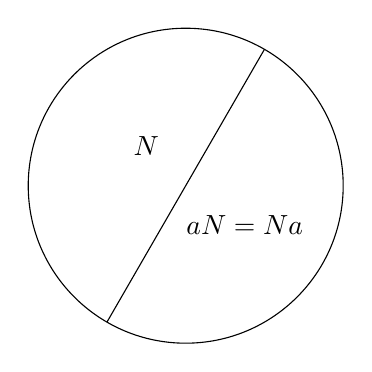
\begin{tikzpicture}
    \draw (0,0) circle [radius=2];
    \draw (-1,{-sqrt(3)}) -- (1,{sqrt(3)});
    \node at (-0.5,0.5) {$N$};
    \node at (0.75,-0.5) {$aN=Na$};
  \end{tikzpicture}
\end{minipage}

\subsection*{1.5.2}

Let $\{N_i\mid i\in I\}$ be a family of normal subgroups of $G$. \\
Prove: $\bigcap_{i\in I}N_i\n G$

Let $N=\bigcap_{i\in I}N_i$ \\
Assume $g\in G$ \\
Assume $n\in N$ \\
$\forall\,i\in I,n\in N_i$ \\
$\forall\,i\in I,gng^{-1}\in N_i$, since $N_i\n G$ \\
So $gng^{-1}\in N$ \\
$\therefore N\n G$

\subsection*{1.5.5}

Let $N=\{\o\in S_4\mid\o(4)=4\}$ \\
Is $N\n G$?

No.  Here is a counterexample:

Let $\o=(12)\in N$ \\
Let $g=(14)\in S_4$ \\
$g^{-1}=(14)$ \\
$g\o g^{-1}=(14)(12)(14)=(24)\notin N$

\subsection*{1.5.6}

Let $H<G$. \\
Prove: $\forall\,a\in G,aHa^{-1}<G$ and $H\simeq aHa^{-1}$

Assume $a\in G$

Assume $h_1,h_2\in H$ \\
By closure, $h_1h_2\in H$ \\
$(ah_1a^{-1})(ah_2a^{-1})=ah_1h_2a^{-1}\in aHa^{-1}$ \\
$\therefore aHa^{-1}$ is closed under the operation.

$e\in H$ \\
$aea^{-1}=aa^{-1}=e$ \\
$e\in aHa^{-1}$ \\
$\therefore aHa^{-1}$ has the identity.

Assume $h\in H$ \\
$h^{-1}\in H$ \\
$ah^{-1}a^{-1}\in aHa^{-1}$ \\
$(aha^{-1})(ah^{-1}a^{-1})=ahh^{-1}a^{-1}=aa^{-1}=e$ \\
$(ah^{-1}a^{-1})(aha^{-1})=ah^{-1}ha^{-1}=aa^{-1}=e$ \\
$\therefore aHa^{-1}$ is closed under inverses.

$\therefore aHa^{-1}<G$

Now, let $\p_a:H\to aHa^{-1}$ be defined by $\p_a(h)=aha^{-1}$

Assume $\p_a(h_1)=\p_a(h_2)$ \\
$ah_1a^{-1}=ah_2a^{-1}$ \\
So, by left and right cancellation, $h_1=h_2$ \\
$\therefore\p_a$ is one-to-one.

Assume $g\in aHa^{-1}$ \\
$\exists\,h\in H,g=aha^{-1}$ \\
$a^{-1}ga=h$ \\
So $a^{-1}ga\in H$ \\
$\p_a(a^{-1}ga)=a(a^{-1}ga)a^{-1}=g$ \\
$\therefore\p_a$ is onto and thus a bijection.

Assume $h_1,h_2\in H$ \\
By closure, $h_1h_2\in H$ \\
$\p_a(h_1h_2)=ah_1h_2a^{-1}=(ah_1a^{-1})(ah_2a^{-1})=\p_a(h_1)\p_a(h_2)$ \\
$\therefore\p$ is a homomorphism and thus an isomorphism.

$\therefore H\simeq aHa^{-1}$

\subsection*{1.5.7}

Let $G$ be a finite group and $H<G$ where $\abs{H}=n$. \\
Prove: $H$ is the only subgroup of order $n\implies H\n G$

By problem (6): $\forall\,a\in G,aHa^{-1}<G$ and $H\simeq aHa^{-1}$ \\
But $H$ is the only subgroup of order $n$, \\
So $H=aHa^{-1}$ \\
$\therefore H\n G$

\subsection*{1.5.9}

\begin{enumerate}[label={\alph*)}]
\item Let $G$ be a group and $H=Z(G)$. Prove: $H\n G$

  It was previously proven that $H\le G$, so need to show normality.

  Assume $g\in G$ \\
  Assume $h\in H$ \\
  $gh=hg$ \\
  $gH=Hg$ \\
  $\therefore H\n G$

\item Prove: $Z(S_n)=\{()\},n\ge3$

  $()\in S_n$ always commutes with everything, so $()\in Z(S_n)$

  Assume $\o\in S_n,\o\ne()$ \\
  $\exists\,i,j\in[n],i\ne j$ and $\o(i)=j$ \\
  Since $\o$ is a bijection, $\o(j)\ne j$ \\
  Since $n\ge3$, $\exists\,k\in[n],k\ne j$ and $k\ne\o(j)$ \\
  Let $\t=(jk)\in S_n$ \\
  Let $\o(j)=\ell$ \\
  $\ell\ne j$ and $\ell\ne k$ \\
  $(\t\o)(j)=\t(\o(j))=\t(\ell)=\ell=\o(j)$ \\
  $(\o\t)(j)=\o(\t(j))=\o(k)$ \\
  But $\o$ is a permutation, and thus a bijection, and thus one-to-one \\
  $j\ne k\implies\o(j)\ne\o(k)$ \\
  $\t\o\ne\o\t$ \\
  So $\o\notin Z(S_n)$
  
  $\therefore Z(S_n)=\{e\}$
\end{enumerate}

\subsection*{1.5.12}

Let $H\n G$ such that $H$ and $G/H$ are finitely-generated. \\
Prove: $G$ is finitely-generated

Let $H=\cycle{X}$ where $X=\{x_1,\ldots,x_r\}$ \\
Let $G/H=\cycle{Y}$ where $Y=\{y_1H,\ldots,y_sH\}$, such that the $y_i$ are the
selected representatives of each left coset in the generating set \\
Since the cosets partition $G$: \\
$G=\bigcup gH=\bigcup\prod(y_iH)^{n_i}=\bigcup\left(\prod y_i^{n_i}\right)H=
\bigcup\left(\prod y_i^{n_i}\right)\left(\prod x_j^{m_j}\right)$ \\
So $G=\cycle{X\cup Y}$ \\
But $X$ and $Y$ finite$\implies X\cup Y$ finite \\
Therefore $G$ is finitely-generated

\subsection*{1.5.16}

Let $f:G\to H$ be a homomorphism of groups, $H$ is abelian, and
$\ker(f)\le N\le G$. \\
Prove: $N\n G$

Let $K=\ker(f)$ \\
$f[G]\le H$ and so $f[G]$ is abelian \\
But by the FIT, $f[G]\simeq G/K$ \\
So $G/K$ is also abelian \\
Assume $g\in G$ \\
Assume $n\in N$ \\
$(gK)nK(g^{-1}K)=(gK)(g^{-1}K)nK=(eK)(nK)=nK$ \\
Thus $N/K\n G/K$ \\
Therefore, by Cor 5.12, $N\n G$

\subsection*{1.5.19}

Let $N\n G$, $(G:N)$ finite, $H<G$, $\abs{H}$ finite, and $((G:N),\abs{H})=1$.
Prove: $H\le N$

Since $N\n G$, $HN\le G$. This results in the following subgroup relationships:

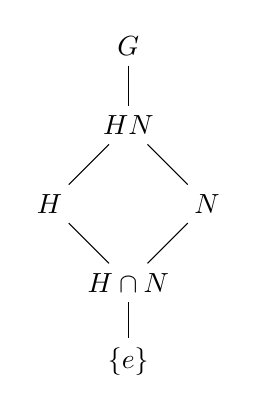
\begin{tikzpicture}
  \node (G) at (2,4) {$G$};
  \node (HN) at (2,3) {$HN$};
  \node (H) at (1,2) {$H$};
  \node (N) at (3,2) {$N$};
  \node (HiN) at (2,1) {$H\cap N$};
  \node (e) at (2,0) {$\{e\}$};
  \path (G) edge (HN);
  \path (HN) edge (H);
  \path (HN) edge (N);
  \path (H) edge (HiN);
  \path (N) edge (HiN);
  \path (HiN) edge (e);
\end{tikzpicture}

$(G:N)=(G:HN)(HN:N)$ \\
$(HN:N)=(H:H\cap N)$\hspace{0.25in}(prop I.4.8) \\
$(G:N)=(G:HN)(H:H\cap N)$

$\abs{H}=(H:\{e\})=(H:H\cap N)(H\cap N:\{e\})$

$((G:N),\abs{H})=((G:HN)(H:H\cap N),(H:H\cap N)(H\cap N:\{e\}))=1$ \\
So $(H:H\cap N)=1$, meaning $H=H\cap N$ \\
$\therefore H\le N$
\end{document}
